\clearpage
\section*{S19. Frozen-state matched-history reuse protocol}
This experiment solves the complete material normal equation at saved states; it does not generate a new nonlinear reconstruction dataset. The common state includes the current factorization, material tangent, retained current basis, and baseline inverse. The prescribed residual sequence contains eight independent seeded complex Gaussian perturbations, each with norm 1\% of the fixed measured-data norm. The same perturbation is used by all methods. Middle-state histories come from the initial saved state; late-state histories come from the middle saved state.

To isolate preconditioning from initialization, every route receives a preceding converged full-normal step computed in a common preparation sequence. Preparation is timed separately. This paired-start contract is stronger than comparing each method from a different warm start, but it is not a deployable autonomous trajectory. Full experiment accounting includes this preparation; marginal-use accounting assumes the shared starts and paid histories exist. A separate history-acquisition surcharge shows what happens if the previous solve must be purchased for reuse. This surcharge is measured once with the common instrumented history collector, which saves both material directions and current snapshots; it is not a separately optimized cold-start collector for each method. The timed target-state plain baseline saves no unnecessary current snapshots.

The plain baseline never saves current snapshots during a timed solve. The current-derived inverse uses at most twelve columns obtained from the previous state's adjoint-current snapshots. Its construction is frozen for all eight right-hand sides. An eight-probe diagnostic is charged once, regardless of whether its sufficient condition passes. The initial six paid full-H actions supply history; they can include the initial-guess action and must not all be called search directions.

\begin{figure}[htbp]\centering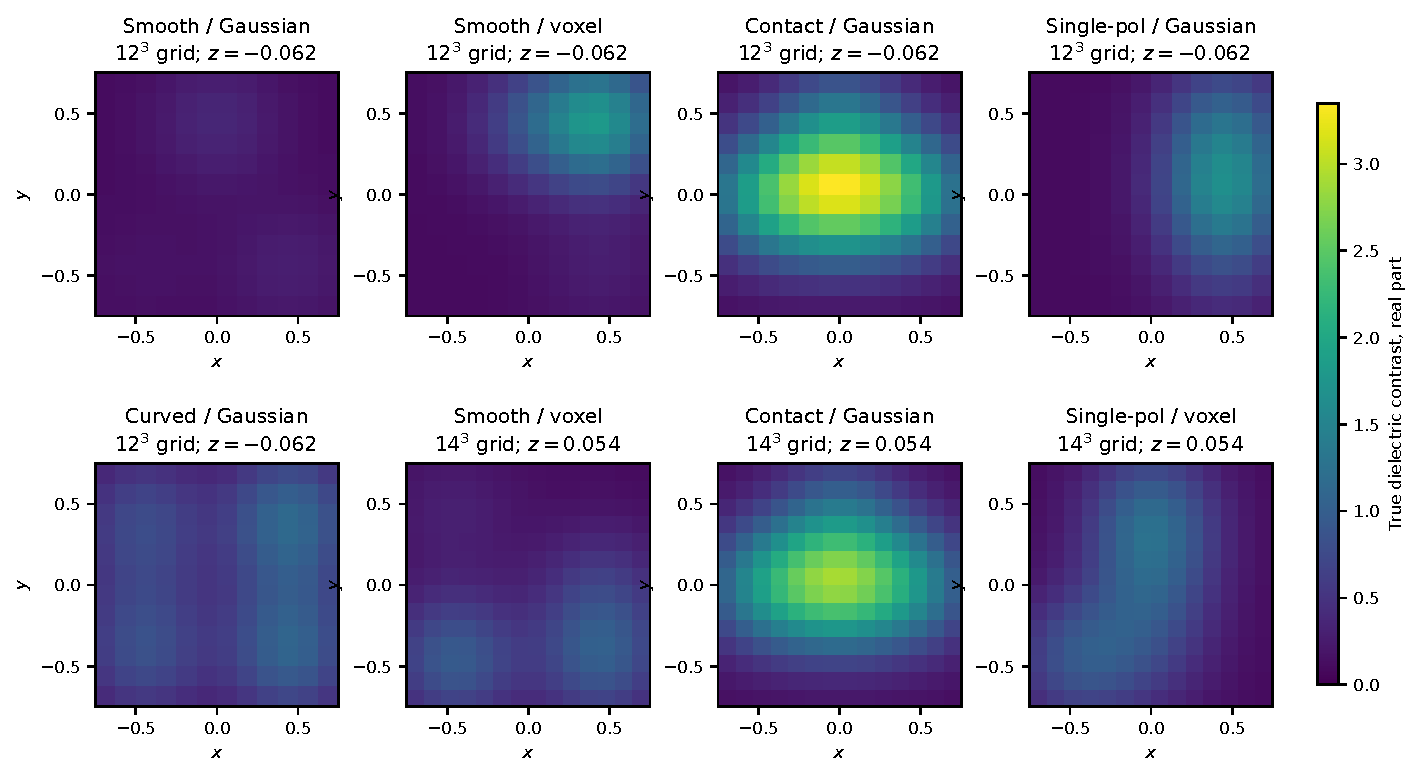
\includegraphics[width=\linewidth]{figures/frozen_objects.pdf}
\caption{Saved target slices for the eight smooth-object cases, using one common real-contrast color scale. These are target fields, not reconstructions. The nearest sampled central $z$ plane is reported for each grid. Gaussian/voxel labels refer to the material tangent used in inversion; ``Single-pol'' changes illumination polarization, not receiver aperture. These are distinct existing objects, so the panels are not a matched representation comparison.}
\end{figure}

\subsection*{State and history separation}
The eight smooth-object saved states use scalar regularization 0.00301 at index 3 and 0.00091 at index 7. Their current banks come from indices 0 and 3, respectively. In the volume-weighted material norm, the relative change from the historical material to the target material ranges from 0.963 to 7.911 for the former pair and from 0.0346 to 0.1512 for the latter. Consequently, an intermediate/late performance difference changes both damping and the proximity of the available history; it does not isolate either as its cause. The two sharp stress states use the same late-state regularization, with relative historical-material changes 0.317 and 0.192. These are extracted state descriptors, not new forward solves or input to the frozen selection rule; the full values are in \texttt{ANCHOR\_STATE\_METADATA.csv}.

\subsection*{Standard material-space two-level comparison}
Let $Z$ contain retained real material directions and $E=Z^THZ$. Define
\[
P=I-ZE^{-1}Z^TH,\qquad
M_{\mathrm{two}}=ZE^{-1}Z^T+PM_0P^T.
\]
For a positive-definite $H,M_0$ and independent $Z$, this inverse action is symmetric positive definite and $M_{\mathrm{two}}HZ=Z$. The implementation applies the two coarse projections and the base inverse without forming $P$. The coarse space is constant throughout a PCG solve. Only after that solve does the method append its own newly paid material directions and reselect generalized Ritz directions using the projected pair $(Z^THZ,Z^TH_0Z)$.

This is a balanced two-level/deflated preconditioner. The general augmentation/deflation framework explains its connection to projected Krylov correction; the code is not claimed to reproduce every singular projected solver in that literature. A separate recent-six coarse warm-start control applies a correction only to the starting vector and is labeled accordingly.

The storage budget equals the current method's extra persistent numerical arrays, excluding references to the common state and baseline inverse. The material method stores $Z,HZ,E$ and its Cholesky factor; the cached sensitivity also includes retained Ritz values. Actual ranks are recorded because a complex current column and a real material column have different dimensions and costs. On a 54-dimensional Gaussian material tangent, this byte budget can eventually admit all 54 directions. Such a full-rank projected spectrum is learned from paid actions, not supplied by an offline oracle. Temporary history and factorization memory are recorded separately from persistent storage.

\subsection*{Finite precision and the cached-image sensitivity}
For nearly dependent columns, forming $HZV\Sigma^{-1}$ can amplify roundoff. A robust realization recomputes $H$ on the rank-revealed basis; all these actions and the associated wall time are charged. Local tests on SPD, clustered, exactly rank-deficient, and nearly dependent histories give coarse-exactness errors below $2.1\times10^{-13}$ across relative dependency scales from $10^{-4}$ to $10^{-14}$.

The separately named cached-image sensitivity uses a stronger normalized singular-value cutoff of $10^{-6}$. Historical images from a different state are refreshed once. Same-state reselection reuses already paid $HZ$, with up to four deterministic orthonormal span checks. An image discrepancy exceeding $10^{-9}\lambda$ times the checked direction norm triggers a paid complete retained-basis refresh. The check is a numerical consistency guard, not a certificate over untested directions. No diagonal jitter is inserted to hide an indefinite coarse matrix.

The cached implementation is reported separately because it changes the numerical realization and the rank cutoff. Its rule was fixed using development evidence before examining validation outcomes. The robust implementation remains in the raw record. A timing lower bound that removes maintenance is explicitly an optimistic sensitivity, not an implemented method.

\subsection*{What the charged Gaussian check certifies}
The repeated-solve experiment checks a normalized Hessian difference, rather than directly estimating the Jacobian-tail quantity $\eta_U$. With $M_C=FF^T$, let $A=F^T(H-H_C)F$. Eight independently generated standard real Gaussian vectors give
\[
\widehat\epsilon_H=2\max_{1\le j\le8}\|Ag_j\|.
\]
For a fixed candidate independent of these probes, the probability that $\widehat\epsilon_H<\|A\|_2$ is at most $\Pr(|N(0,1)|<1/2)^8\simeq4.62\times10^{-4}$. If the bound is below1, the symmetric preconditioned spectrum lies in $[1-\widehat\epsilon_H,1+\widehat\epsilon_H]$ with that probability guarantee. An acceptance flag uses the stricter threshold0.6. Performance measurements still run the SPD inverse when the flag rejects, so they are empirical tests rather than a certified deployment policy.

The five timing repetitions reuse the same fixed probes and candidate, and are not five independent probability events. Across18 distinct tested frozen states, a union bound is at most0.00833; it is conservative and does not claim probe completeness. Construction of the inverse square-root factors and all eight full-H actions are charged. The full-Hessian check and the earlier regularization-whitened Jacobian bounds are separate quantities in the evidence record.

\subsection*{Stopping, timing, and units of evidence}
All timed routes use FP64, the same full $H,h$, regularization, and relative true normal residual threshold $10^{-8}$. PCG has at most 150 steps and checks the actual residual, with replacement if a recursive residual is misleading. Every row records achieved residual, full-wave right-hand sides, setup, application, capture, reselection, and total time. Small-system spectra and exact full spectra used for interpretation are excluded from online selection and separately charged.

Five repetitions use identical physical data and rotate method order. Their median and interquartile range quantify timing variability. Eight noise residuals are eight uses of one state, not independent objects. Middle and late states of one object are also correlated. Overall validation summaries aggregate at object level. Development objects, six rule-validation objects, and two sharp stress objects remain distinct groups.

A sustained break-even use is the first use after which cumulative current-method cost remains below matched baseline cost through the eighth use. It includes construction and the diagnostic check. An absent break-even is recorded, not extrapolated from average iteration savings. If history is not already available, its measured acquisition cost is added as a separate surcharge. Initial geometry/operator assembly and experiment bookkeeping are also contained in the complete monitored job time, but are not isolated as separately repeated per-method phases. Accordingly, route comparisons are labeled marginal or paired-common-cost comparisons; the occupation ledger gives the total campaign expenditure, not an autonomous cold-start speedup.

\noindent Ratios compare eight complete solves with the same-phase baseline. Cost cells give median [Q1,Q3] over five timing repetitions. Paid history adds the previous-state instrumented history acquisition. All quality outcomes are retained.
\par Rank labels: C/W are complex current/signature ranks; R is the real material coarse rank. They are different spaces. Diagnostic counts and KiB are medians; the machine-readable record retains every repetition. Sustained break-even (BE) is the number of successful repetitions followed by the minimum--maximum use index.
\par\medskip\noindent\begin{minipage}{\linewidth}\textbf{Development --- Paid-refresh Ritz (part 1)}
\begin{center}\fontsize{8}{10}\selectfont\setlength{\tabcolsep}{3pt}
\resizebox{\textwidth}{!}{\begin{tabular}{llccc}
\toprule Case/state & Method & Available history ratio & History charged ratio & History (s)\\\midrule
Smooth G12 / mid & Current & 0.998 [0.995,1.004] & 1.420 [1.418,1.431] & 4.49\\
Smooth G12 / mid & Ritz & 3.676 [3.651,3.684] & 4.098 [4.072,4.111] & 4.49\\
Smooth G12 / mid & Warm start & 1.153 [1.141,1.159] & 1.575 [1.561,1.585] & 4.49\\
Smooth G12 / late & Current & 0.802 [0.802,0.805] & 1.197 [1.196,1.203] & 5.32\\
Smooth G12 / late & Ritz & 2.851 [2.836,2.872] & 3.248 [3.232,3.266] & 5.32\\
Smooth G12 / late & Warm start & 1.110 [1.109,1.110] & 1.506 [1.504,1.506] & 5.32\\
Smooth V12 / mid & Current & 1.000 [0.998,1.004] & 1.278 [1.272,1.281] & 4.88\\
Smooth V12 / mid & Ritz & 3.633 [3.625,3.634] & 3.911 [3.900,3.912] & 4.88\\
Smooth V12 / mid & Warm start & 1.082 [1.077,1.086] & 1.357 [1.351,1.363] & 4.88\\
Smooth V12 / late & Current & 0.733 [0.731,0.738] & 0.989 [0.982,0.996] & 6.07\\
Smooth V12 / late & Ritz & 3.374 [3.356,3.382] & 3.630 [3.610,3.638] & 6.07\\
Smooth V12 / late & Warm start & 1.052 [1.046,1.054] & 1.307 [1.300,1.310] & 6.07\\
\bottomrule\end{tabular}}\end{center}
\end{minipage}
\begin{center}\fontsize{8}{10}\selectfont\setlength{\tabcolsep}{3pt}
\resizebox{\textwidth}{!}{\begin{tabular}{llccccc}
\toprule Case/state & Method & Rank & KiB & Full-wave RHS & True residual & Sustained BE\\\midrule
Smooth G12 / mid & Current & C12/W27 & 1445.8 & 1128 & 8.57e-09 & 3/5: 8--8\\
Smooth G12 / mid & Ritz & R4--54 & 91.1 & 5406 & 7.78e-09 & none (0/5)\\
Smooth G12 / mid & Warm start & R4--6 & 5.3 & 1320 & 6.47e-09 & none (0/5)\\
Smooth G12 / late & Current & C12/W27 & 1445.8 & 1152 & 2.63e-09 & 5/5: 3--3\\
Smooth G12 / late & Ritz & R6--54 & 91.1 & 5286 & 8.98e-09 & none (0/5)\\
Smooth G12 / late & Warm start & R6--6 & 5.3 & 1608 & 7.22e-09 & none (0/5)\\
Smooth V12 / mid & Current & C12/W144 & 16226.6 & 1632 & 8.74e-09 & 3/5: 8--8\\
Smooth V12 / mid & Ritz & R6--88 & 4873.0 & 8796 & 6.76e-09 & none (0/5)\\
Smooth V12 / mid & Warm start & R6--6 & 324.3 & 1992 & 7.88e-09 & none (0/5)\\
Smooth V12 / late & Current & C12/W144 & 16226.6 & 1620 & 7.22e-09 & 5/5: 2--3\\
Smooth V12 / late & Ritz & R6--110 & 6129.1 & 11016 & 7.24e-09 & none (0/5)\\
Smooth V12 / late & Warm start & R6--6 & 324.3 & 2604 & 9.29e-09 & none (0/5)\\
\bottomrule\end{tabular}}\end{center}
\par\medskip\noindent\begin{minipage}{\linewidth}\textbf{Development --- Cached-image Ritz (part 1)}
\begin{center}\fontsize{8}{10}\selectfont\setlength{\tabcolsep}{3pt}
\resizebox{\textwidth}{!}{\begin{tabular}{llccc}
\toprule Case/state & Method & Available history ratio & History charged ratio & History (s)\\\midrule
Smooth G12 / mid & Current & 0.998 [0.996,0.999] & 1.430 [1.430,1.432] & 4.77\\
Smooth G12 / mid & Ritz & 1.122 [1.122,1.124] & 1.555 [1.554,1.556] & 4.77\\
Smooth G12 / late & Current & 0.808 [0.807,0.809] & 1.203 [1.202,1.205] & 5.50\\
Smooth G12 / late & Ritz & 0.918 [0.917,0.919] & 1.311 [1.310,1.316] & 5.50\\
Smooth V12 / mid & Current & 1.012 [1.011,1.015] & 1.292 [1.290,1.293] & 5.08\\
Smooth V12 / mid & Ritz & 0.986 [0.984,0.986] & 1.264 [1.263,1.264] & 5.08\\
Smooth V12 / late & Current & 0.740 [0.740,0.741] & 0.997 [0.996,0.998] & 6.35\\
Smooth V12 / late & Ritz & 0.858 [0.855,0.859] & 1.115 [1.111,1.115] & 6.35\\
\bottomrule\end{tabular}}\end{center}
\end{minipage}
\begin{center}\fontsize{8}{10}\selectfont\setlength{\tabcolsep}{3pt}
\resizebox{\textwidth}{!}{\begin{tabular}{llccccc}
\toprule Case/state & Method & Rank & KiB & Full-wave RHS & True residual & Sustained BE\\\midrule
Smooth G12 / mid & Current & C12/W27 & 1445.8 & 1128 & 8.57e-09 & 5/5: 8--8\\
Smooth G12 / mid & Ritz & R4--50 & 81.6 & 1440 & 7.78e-09 & none (0/5)\\
Smooth G12 / late & Current & C12/W27 & 1445.8 & 1152 & 2.63e-09 & 5/5: 3--3\\
Smooth G12 / late & Ritz & R6--54 & 91.5 & 1488 & 8.98e-09 & 5/5: 8--8\\
Smooth V12 / mid & Current & C12/W144 & 16226.6 & 1632 & 8.74e-09 & none (0/5)\\
Smooth V12 / mid & Ritz & R6--83 & 4590.3 & 1896 & 7.51e-09 & 5/5: 8--8\\
Smooth V12 / late & Current & C12/W144 & 16226.6 & 1620 & 7.22e-09 & 5/5: 3--3\\
Smooth V12 / late & Ritz & R6--106 & 5900.4 & 2196 & 9.00e-09 & 5/5: 5--5\\
\bottomrule\end{tabular}}\end{center}
\par\medskip\noindent\begin{minipage}{\linewidth}\textbf{Validation --- Paid-refresh Ritz (part 1)}
\begin{center}\fontsize{8}{10}\selectfont\setlength{\tabcolsep}{3pt}
\resizebox{\textwidth}{!}{\begin{tabular}{llccc}
\toprule Case/state & Method & Available history ratio & History charged ratio & History (s)\\\midrule
Contact G12 / mid & Current & 0.951 [0.945,0.955] & 1.291 [1.285,1.299] & 4.82\\
Contact G12 / mid & Ritz & 2.255 [2.246,2.258] & 2.595 [2.587,2.601] & 4.82\\
Contact G12 / mid & Warm start & 1.111 [1.106,1.119] & 1.452 [1.446,1.462] & 4.82\\
Contact G12 / late & Current & 0.684 [0.679,0.691] & 0.993 [0.991,1.003] & 5.54\\
Contact G12 / late & Ritz & 1.669 [1.651,1.670] & 1.981 [1.959,1.983] & 5.54\\
Contact G12 / late & Warm start & 1.087 [1.084,1.091] & 1.397 [1.392,1.402] & 5.54\\
Single-pol G12 / mid & Current & 0.909 [0.895,0.911] & 1.249 [1.235,1.254] & 4.86\\
Single-pol G12 / mid & Ritz & 2.765 [2.748,2.768] & 3.107 [3.085,3.108] & 4.86\\
Single-pol G12 / mid & Warm start & 1.112 [1.104,1.115] & 1.452 [1.447,1.453] & 4.86\\
Single-pol G12 / late & Current & 0.716 [0.714,0.716] & 1.079 [1.078,1.080] & 5.59\\
Single-pol G12 / late & Ritz & 2.613 [2.613,2.614] & 2.976 [2.976,2.978] & 5.59\\
Single-pol G12 / late & Warm start & 1.086 [1.083,1.091] & 1.451 [1.449,1.454] & 5.59\\
\bottomrule\end{tabular}}\end{center}
\end{minipage}
\begin{center}\fontsize{8}{10}\selectfont\setlength{\tabcolsep}{3pt}
\resizebox{\textwidth}{!}{\begin{tabular}{llccccc}
\toprule Case/state & Method & Rank & KiB & Full-wave RHS & True residual & Sustained BE\\\midrule
Contact G12 / mid & Current & C12/W27 & 1445.8 & 1428 & 6.99e-09 & 5/5: 5--6\\
Contact G12 / mid & Ritz & R6--54 & 91.1 & 4350 & 7.90e-09 & none (0/5)\\
Contact G12 / mid & Warm start & R6--6 & 5.3 & 1692 & 7.05e-09 & none (0/5)\\
Contact G12 / late & Current & C12/W27 & 1445.8 & 1296 & 9.72e-09 & 5/5: 2--2\\
Contact G12 / late & Ritz & R6--54 & 91.1 & 4020 & 3.97e-09 & none (0/5)\\
Contact G12 / late & Warm start & R6--6 & 5.3 & 2088 & 8.70e-09 & none (0/5)\\
Single-pol G12 / mid & Current & C12/W27 & 1445.8 & 1368 & 8.32e-09 & 5/5: 4--4\\
Single-pol G12 / mid & Ritz & R6--54 & 91.1 & 5424 & 3.82e-09 & none (0/5)\\
Single-pol G12 / mid & Warm start & R6--6 & 5.3 & 1704 & 3.31e-09 & none (0/5)\\
Single-pol G12 / late & Current & C12/W27 & 1445.8 & 1152 & 8.67e-09 & 5/5: 2--2\\
Single-pol G12 / late & Ritz & R6--54 & 91.1 & 5508 & 9.83e-09 & none (0/5)\\
Single-pol G12 / late & Warm start & R6--6 & 5.3 & 1788 & 9.76e-09 & none (0/5)\\
\bottomrule\end{tabular}}\end{center}
\par\medskip\noindent\begin{minipage}{\linewidth}\textbf{Validation --- Paid-refresh Ritz (part 2)}
\begin{center}\fontsize{8}{10}\selectfont\setlength{\tabcolsep}{3pt}
\resizebox{\textwidth}{!}{\begin{tabular}{llccc}
\toprule Case/state & Method & Available history ratio & History charged ratio & History (s)\\\midrule
Curved G12 / mid & Current & 0.835 [0.834,0.838] & 1.168 [1.167,1.169] & 4.88\\
Curved G12 / mid & Ritz & 2.259 [2.258,2.261] & 2.592 [2.591,2.592] & 4.88\\
Curved G12 / mid & Warm start & 1.111 [1.109,1.111] & 1.442 [1.439,1.443] & 4.88\\
Curved G12 / late & Current & 0.710 [0.704,0.714] & 1.029 [1.023,1.031] & 5.33\\
Curved G12 / late & Ritz & 2.119 [2.065,2.119] & 2.438 [2.378,2.442] & 5.33\\
Curved G12 / late & Warm start & 1.095 [1.062,1.095] & 1.413 [1.377,1.418] & 5.33\\
Smooth V14 / mid & Current & 0.944 [0.943,0.949] & 1.326 [1.326,1.330] & 13.45\\
Smooth V14 / mid & Ritz & 3.605 [3.605,3.611] & 3.987 [3.985,3.993] & 13.45\\
Smooth V14 / mid & Warm start & 1.080 [1.079,1.082] & 1.462 [1.461,1.463] & 13.45\\
Smooth V14 / late & Current & 0.720 [0.719,0.720] & 1.058 [1.057,1.059] & 15.67\\
Smooth V14 / late & Ritz & 3.445 [3.443,3.450] & 3.783 [3.782,3.788] & 15.67\\
Smooth V14 / late & Warm start & 1.047 [1.047,1.048] & 1.386 [1.386,1.386] & 15.67\\
\bottomrule\end{tabular}}\end{center}
\end{minipage}
\begin{center}\fontsize{8}{10}\selectfont\setlength{\tabcolsep}{3pt}
\resizebox{\textwidth}{!}{\begin{tabular}{llccccc}
\toprule Case/state & Method & Rank & KiB & Full-wave RHS & True residual & Sustained BE\\\midrule
Curved G12 / mid & Current & C12/W27 & 1445.8 & 1260 & 8.22e-09 & 5/5: 3--3\\
Curved G12 / mid & Ritz & R5--54 & 91.1 & 4374 & 9.16e-09 & none (0/5)\\
Curved G12 / mid & Warm start & R5--6 & 5.3 & 1704 & 2.46e-09 & none (0/5)\\
Curved G12 / late & Current & C12/W27 & 1445.8 & 1212 & 8.42e-09 & 5/5: 2--2\\
Curved G12 / late & Ritz & R6--54 & 91.1 & 4674 & 9.95e-09 & none (0/5)\\
Curved G12 / late & Warm start & R6--6 & 5.3 & 1896 & 5.23e-09 & none (0/5)\\
Smooth V14 / mid & Current & C12/W144 & 25370.6 & 1728 & 4.80e-09 & 5/5: 6--6\\
Smooth V14 / mid & Ritz & R6--96 & 8376.0 & 9504 & 7.47e-09 & none (0/5)\\
Smooth V14 / mid & Warm start & R6--6 & 514.8 & 2196 & 7.17e-09 & none (0/5)\\
Smooth V14 / late & Current & C12/W144 & 25370.6 & 1728 & 7.02e-09 & 5/5: 2--2\\
Smooth V14 / late & Ritz & R6--119 & 10425.5 & 11934 & 8.98e-09 & none (0/5)\\
Smooth V14 / late & Warm start & R6--6 & 514.8 & 2796 & 9.79e-09 & none (0/5)\\
\bottomrule\end{tabular}}\end{center}
\par\medskip\noindent\begin{minipage}{\linewidth}\textbf{Validation --- Paid-refresh Ritz (part 3)}
\begin{center}\fontsize{8}{10}\selectfont\setlength{\tabcolsep}{3pt}
\resizebox{\textwidth}{!}{\begin{tabular}{llccc}
\toprule Case/state & Method & Available history ratio & History charged ratio & History (s)\\\midrule
Contact G14 / mid & Current & 0.923 [0.922,0.925] & 1.382 [1.382,1.386] & 12.93\\
Contact G14 / mid & Ritz & 2.218 [2.215,2.219] & 2.678 [2.674,2.680] & 12.93\\
Contact G14 / mid & Warm start & 1.086 [1.086,1.086] & 1.546 [1.546,1.546] & 12.93\\
Contact G14 / late & Current & 0.658 [0.656,0.658] & 1.084 [1.082,1.086] & 14.64\\
Contact G14 / late & Ritz & 1.613 [1.611,1.614] & 2.040 [2.037,2.041] & 14.64\\
Contact G14 / late & Warm start & 1.066 [1.064,1.067] & 1.493 [1.490,1.494] & 14.64\\
Single-pol V14 / mid & Current & 1.096 [1.091,1.098] & 1.480 [1.474,1.481] & 12.97\\
Single-pol V14 / mid & Ritz & 3.954 [3.951,3.959] & 4.338 [4.336,4.342] & 12.97\\
Single-pol V14 / mid & Warm start & 1.072 [1.072,1.074] & 1.457 [1.456,1.458] & 12.97\\
Single-pol V14 / late & Current & 0.719 [0.719,0.721] & 1.050 [1.049,1.053] & 15.47\\
Single-pol V14 / late & Ritz & 3.755 [3.755,3.757] & 4.087 [4.086,4.088] & 15.47\\
Single-pol V14 / late & Warm start & 1.039 [1.039,1.040] & 1.371 [1.370,1.371] & 15.47\\
\bottomrule\end{tabular}}\end{center}
\end{minipage}
\begin{center}\fontsize{8}{10}\selectfont\setlength{\tabcolsep}{3pt}
\resizebox{\textwidth}{!}{\begin{tabular}{llccccc}
\toprule Case/state & Method & Rank & KiB & Full-wave RHS & True residual & Sustained BE\\\midrule
Contact G14 / mid & Current & C12/W27 & 2017.3 & 1512 & 8.46e-09 & 5/5: 5--5\\
Contact G14 / mid & Ritz & R6--54 & 91.1 & 4608 & 7.64e-09 & none (0/5)\\
Contact G14 / mid & Warm start & R6--6 & 5.3 & 1800 & 7.14e-09 & none (0/5)\\
Contact G14 / late & Current & C12/W27 & 2017.3 & 1308 & 7.89e-09 & 5/5: 2--2\\
Contact G14 / late & Ritz & R6--54 & 91.1 & 4038 & 4.69e-09 & none (0/5)\\
Contact G14 / late & Warm start & R6--6 & 5.3 & 2148 & 9.28e-09 & none (0/5)\\
Single-pol V14 / mid & Current & C12/W144 & 25370.6 & 1920 & 5.43e-09 & none (0/5)\\
Single-pol V14 / mid & Ritz & R6--104 & 9087.0 & 9948 & 9.78e-09 & none (0/5)\\
Single-pol V14 / mid & Warm start & R6--6 & 514.8 & 2088 & 7.79e-09 & none (0/5)\\
Single-pol V14 / late & Current & C12/W144 & 25370.6 & 1740 & 9.49e-09 & 5/5: 2--2\\
Single-pol V14 / late & Ritz & R6--134 & 11771.1 & 13086 & 8.41e-09 & none (0/5)\\
Single-pol V14 / late & Warm start & R6--6 & 514.8 & 2796 & 9.48e-09 & none (0/5)\\
\bottomrule\end{tabular}}\end{center}
\par\medskip\noindent\begin{minipage}{\linewidth}\textbf{Validation --- Cached-image Ritz (part 1)}
\begin{center}\fontsize{8}{10}\selectfont\setlength{\tabcolsep}{3pt}
\resizebox{\textwidth}{!}{\begin{tabular}{llccc}
\toprule Case/state & Method & Available history ratio & History charged ratio & History (s)\\\midrule
Contact G12 / mid & Current & 0.950 [0.948,0.952] & 1.293 [1.288,1.294] & 5.01\\
Contact G12 / mid & Ritz & 0.850 [0.849,0.853] & 1.193 [1.193,1.194] & 5.01\\
Contact G12 / late & Current & 0.686 [0.684,0.686] & 1.008 [1.006,1.012] & 6.00\\
Contact G12 / late & Ritz & 0.628 [0.628,0.630] & 0.951 [0.950,0.952] & 6.00\\
Single-pol G12 / mid & Current & 0.907 [0.906,0.908] & 1.219 [1.217,1.220] & 4.56\\
Single-pol G12 / mid & Ritz & 0.842 [0.841,0.844] & 1.155 [1.152,1.156] & 4.56\\
Single-pol G12 / late & Current & 0.718 [0.718,0.720] & 1.102 [1.102,1.103] & 5.96\\
Single-pol G12 / late & Ritz & 0.791 [0.790,0.791] & 1.174 [1.174,1.175] & 5.96\\
Curved G12 / mid & Current & 0.835 [0.833,0.837] & 1.168 [1.165,1.172] & 4.90\\
Curved G12 / mid & Ritz & 0.842 [0.841,0.843] & 1.177 [1.171,1.178] & 4.90\\
Curved G12 / late & Current & 0.716 [0.716,0.718] & 1.072 [1.069,1.072] & 5.82\\
Curved G12 / late & Ritz & 0.726 [0.724,0.726] & 1.080 [1.078,1.081] & 5.82\\
\bottomrule\end{tabular}}\end{center}
\end{minipage}
\begin{center}\fontsize{8}{10}\selectfont\setlength{\tabcolsep}{3pt}
\resizebox{\textwidth}{!}{\begin{tabular}{llccccc}
\toprule Case/state & Method & Rank & KiB & Full-wave RHS & True residual & Sustained BE\\\midrule
Contact G12 / mid & Current & C12/W27 & 1445.8 & 1428 & 6.99e-09 & 5/5: 5--6\\
Contact G12 / mid & Ritz & R6--54 & 91.5 & 1428 & 7.90e-09 & 5/5: 7--7\\
Contact G12 / late & Current & C12/W27 & 1445.8 & 1296 & 9.72e-09 & 5/5: 2--2\\
Contact G12 / late & Ritz & R6--54 & 91.5 & 1308 & 3.97e-09 & 5/5: 5--5\\
Single-pol G12 / mid & Current & C12/W27 & 1445.8 & 1368 & 8.32e-09 & 5/5: 4--4\\
Single-pol G12 / mid & Ritz & R6--54 & 91.5 & 1428 & 5.38e-09 & 5/5: 7--7\\
Single-pol G12 / late & Current & C12/W27 & 1445.8 & 1152 & 8.67e-09 & 5/5: 2--2\\
Single-pol G12 / late & Ritz & R6--54 & 91.5 & 1428 & 3.95e-09 & 5/5: 6--6\\
Curved G12 / mid & Current & C12/W27 & 1445.8 & 1260 & 8.22e-09 & 5/5: 3--3\\
Curved G12 / mid & Ritz & R5--54 & 91.5 & 1422 & 9.16e-09 & 5/5: 7--7\\
Curved G12 / late & Current & C12/W27 & 1445.8 & 1212 & 8.42e-09 & 5/5: 2--2\\
Curved G12 / late & Ritz & R6--54 & 91.5 & 1368 & 9.66e-09 & 5/5: 6--6\\
\bottomrule\end{tabular}}\end{center}
\par\medskip\noindent\begin{minipage}{\linewidth}\textbf{Validation --- Cached-image Ritz (part 2)}
\begin{center}\fontsize{8}{10}\selectfont\setlength{\tabcolsep}{3pt}
\resizebox{\textwidth}{!}{\begin{tabular}{llccc}
\toprule Case/state & Method & Available history ratio & History charged ratio & History (s)\\\midrule
Smooth V14 / mid & Current & 0.944 [0.944,0.946] & 1.317 [1.316,1.318] & 13.13\\
Smooth V14 / mid & Ritz & 0.940 [0.939,0.940] & 1.311 [1.311,1.313] & 13.13\\
Smooth V14 / late & Current & 0.722 [0.721,0.723] & 1.062 [1.061,1.062] & 15.71\\
Smooth V14 / late & Ritz & 0.847 [0.847,0.848] & 1.187 [1.186,1.187] & 15.71\\
Contact G14 / mid & Current & 0.925 [0.925,0.925] & 1.380 [1.379,1.381] & 12.83\\
Contact G14 / mid & Ritz & 0.750 [0.749,0.750] & 1.204 [1.204,1.205] & 12.83\\
Contact G14 / late & Current & 0.658 [0.657,0.658] & 1.088 [1.087,1.088] & 14.74\\
Contact G14 / late & Ritz & 0.601 [0.601,0.602] & 1.031 [1.029,1.031] & 14.74\\
Single-pol V14 / mid & Current & 1.096 [1.095,1.096] & 1.480 [1.480,1.480] & 12.99\\
Single-pol V14 / mid & Ritz & 1.053 [1.052,1.053] & 1.437 [1.436,1.438] & 12.99\\
Single-pol V14 / late & Current & 0.719 [0.719,0.720] & 1.051 [1.050,1.052] & 15.53\\
Single-pol V14 / late & Ritz & 0.917 [0.916,0.917] & 1.248 [1.247,1.248] & 15.53\\
\bottomrule\end{tabular}}\end{center}
\end{minipage}
\begin{center}\fontsize{8}{10}\selectfont\setlength{\tabcolsep}{3pt}
\resizebox{\textwidth}{!}{\begin{tabular}{llccccc}
\toprule Case/state & Method & Rank & KiB & Full-wave RHS & True residual & Sustained BE\\\midrule
Smooth V14 / mid & Current & C12/W144 & 25370.6 & 1728 & 4.80e-09 & 5/5: 6--6\\
Smooth V14 / mid & Ritz & R6--91 & 7933.4 & 1992 & 9.48e-09 & 5/5: 8--8\\
Smooth V14 / late & Current & C12/W144 & 25370.6 & 1728 & 7.02e-09 & 5/5: 2--2\\
Smooth V14 / late & Ritz & R6--115 & 10068.8 & 2304 & 8.98e-09 & 5/5: 5--5\\
Contact G14 / mid & Current & C12/W27 & 2017.3 & 1512 & 8.46e-09 & 5/5: 5--5\\
Contact G14 / mid & Ritz & R6--54 & 91.5 & 1356 & 9.52e-09 & 5/5: 6--6\\
Contact G14 / late & Current & C12/W27 & 2017.3 & 1308 & 7.89e-09 & 5/5: 2--2\\
Contact G14 / late & Ritz & R6--54 & 91.5 & 1308 & 4.69e-09 & 5/5: 5--5\\
Single-pol V14 / mid & Current & C12/W144 & 25370.6 & 1920 & 5.43e-09 & none (0/5)\\
Single-pol V14 / mid & Ritz & R6--99 & 8643.2 & 2124 & 9.78e-09 & none (0/5)\\
Single-pol V14 / late & Current & C12/W144 & 25370.6 & 1740 & 9.49e-09 & 5/5: 2--2\\
Single-pol V14 / late & Ritz & R6--129 & 11322.8 & 2496 & 9.17e-09 & 5/5: 7--7\\
\bottomrule\end{tabular}}\end{center}
\par\medskip\noindent\begin{minipage}{\linewidth}\textbf{Sharp stress --- Paid-refresh Ritz (part 1)}
\begin{center}\fontsize{8}{10}\selectfont\setlength{\tabcolsep}{3pt}
\resizebox{\textwidth}{!}{\begin{tabular}{llccc}
\toprule Case/state & Method & Available history ratio & History charged ratio & History (s)\\\midrule
Sharp sphere / late & Current & 0.540 [0.540,0.541] & 0.669 [0.668,0.670] & 8.69\\
Sharp sphere / late & Ritz & 2.552 [2.549,2.553] & 2.681 [2.677,2.682] & 8.69\\
Sharp sphere / late & Warm start & 1.011 [1.009,1.013] & 1.139 [1.138,1.141] & 8.69\\
Layered cuboid / late & Current & 0.465 [0.465,0.467] & 0.613 [0.612,0.614] & 8.91\\
Layered cuboid / late & Ritz & 2.608 [2.605,2.612] & 2.754 [2.752,2.760] & 8.91\\
Layered cuboid / late & Warm start & 1.020 [1.020,1.023] & 1.166 [1.166,1.170] & 8.91\\
\bottomrule\end{tabular}}\end{center}
\end{minipage}
\begin{center}\fontsize{8}{10}\selectfont\setlength{\tabcolsep}{3pt}
\resizebox{\textwidth}{!}{\begin{tabular}{llccccc}
\toprule Case/state & Method & Rank & KiB & Full-wave RHS & True residual & Sustained BE\\\midrule
Sharp sphere / late & Current & C12/W144 & 16226.6 & 3324 & 9.88e-09 & 5/5: 1--1\\
Sharp sphere / late & Ritz & R6--219 & 12575.4 & 22956 & 9.57e-09 & none (0/5)\\
Sharp sphere / late & Warm start & R6--6 & 324.3 & 6864 & 9.28e-09 & none (0/5)\\
Layered cuboid / late & Current & C12/W144 & 16226.6 & 2556 & 9.76e-09 & 5/5: 1--1\\
Layered cuboid / late & Ritz & R6--200 & 11425.0 & 21054 & 9.98e-09 & none (0/5)\\
Layered cuboid / late & Warm start & R6--6 & 324.3 & 6240 & 9.74e-09 & none (0/5)\\
\bottomrule\end{tabular}}\end{center}
\par\medskip\noindent\begin{minipage}{\linewidth}\textbf{Sharp stress --- Cached-image Ritz (part 1)}
\begin{center}\fontsize{8}{10}\selectfont\setlength{\tabcolsep}{3pt}
\resizebox{\textwidth}{!}{\begin{tabular}{llccc}
\toprule Case/state & Method & Available history ratio & History charged ratio & History (s)\\\midrule
Sharp sphere / late & Current & 0.541 [0.540,0.541] & 0.671 [0.670,0.672] & 8.80\\
Sharp sphere / late & Ritz & 0.684 [0.682,0.685] & 0.815 [0.812,0.815] & 8.80\\
Layered cuboid / late & Current & 0.467 [0.467,0.467] & 0.615 [0.615,0.615] & 9.00\\
Layered cuboid / late & Ritz & 0.705 [0.703,0.706] & 0.853 [0.851,0.854] & 9.00\\
\bottomrule\end{tabular}}\end{center}
\end{minipage}
\begin{center}\fontsize{8}{10}\selectfont\setlength{\tabcolsep}{3pt}
\resizebox{\textwidth}{!}{\begin{tabular}{llccccc}
\toprule Case/state & Method & Rank & KiB & Full-wave RHS & True residual & Sustained BE\\\midrule
Sharp sphere / late & Current & C12/W144 & 16226.6 & 3324 & 9.88e-09 & 5/5: 1--1\\
Sharp sphere / late & Ritz & R6--217 & 12455.5 & 4872 & 9.96e-09 & 5/5: 5--5\\
Layered cuboid / late & Current & C12/W144 & 16226.6 & 2556 & 9.76e-09 & 5/5: 1--1\\
Layered cuboid / late & Ritz & R6--197 & 11245.9 & 4542 & 9.39e-09 & 5/5: 5--5\\
\bottomrule\end{tabular}}\end{center}
\noindent Current RHS includes its paid check; Ritz RHS includes image checks and refresh/reselection. History acquisition and common starting-step preparation are separate. The cache does not run the warm-start control. Rank ranges cover uses and repetitions; complex signature rank is not real-material rank. Object-level statistics combine the two correlated states within each timing repetition. Full arrays, timings, and per-stage action counts are in the accompanying CSV/JSON ledger.


\section*{S20. Independent angular sphere reference}
The fixed target has radius 0.35, background wavenumber 2, and contrast $1+0.05i$, centered in a cube of side1.5. The prescribed grid sides are16,20,24,28,32. Only exterior points with exactly zero polarizability are removed. This support restriction defines the forward validation geometry; it is not an unknown-boundary inversion prior.

The reference is a vector Mie series evaluated for arbitrary incidence and transverse observation bases, with time convention $e^{-i\omega t}$, incident phase $e^{ik\widehat u\cdot x}$, and outgoing phase $e^{ikR}/R$. Both references use strict leading far-field reception. All six illuminations and both transverse components at64 directions enter the complex aggregate error. The DDA local kernel and polarizability are not used to generate the analytic reference.

The uniform derivative direction is $\delta\chi=1$ at every active cell, at the stated complex material. Central differences of the Mie series use steps $10^{-4},3\times10^{-5},10^{-5}$; the declared error uses $10^{-5}$ and the Mie derivative norm in the denominator. Richardson extrapolation is a diagnostic only. Some inherited JSON key names contain ``best''; the value is selected by this fixed rule, not by the smallest observed error. The same definition is used in every table.

\begin{center}\begin{tabular}{rrrrr}\toprule
Grid & Active cells & Volume ratio & Field (\%) & Derivative (\%)\\\midrule
16$^3$ & 208 & 0.9543 & 4.169 & 3.605\\
20$^3$ & 432 & 1.0148 & 1.873 & 2.907\\
24$^3$ & 720 & 0.9788 & 1.747 & 1.294\\
28$^3$ & 1088 & 0.9314 & 6.437 & 6.162\\
32$^3$ & 1736 & 0.9956 & 0.252 & 0.731\\
\bottomrule\end{tabular}\end{center}


The aggregate error weights complex components by their actual amplitudes. Maximum angular discrepancy is additionally reported relative to the global reference peak. The phase of a nearly vanishing cross-polarized response is poorly defined: maximum componentwise phase errors can approach $180^\circ$ even when the aggregate vector error is small. The raw record includes the amplitude floor used for that statistic and the amplitude-weighted phase RMS. This is why neither maximum phase nor aggregate error alone substitutes for the full angular comparison.

The $28^3$ grid underrepresents the sphere volume by6.86\%; its nonmonotone error is retained. The finest grid passes the field/derivative targets for this fixed target, while the whole grid sequence does not pass at every resolution. The uniform derivative check does not certify all independent voxel directions. The associated voxel preconditioner and Ritz values are discrete diagnostics, explicitly separated from the analytic uniform-sphere comparison.

\section*{S21. Candidate scoring without full-Jacobian selection}
At each prescribed late state, a pool combines twelve receiver directions, twelve internal-propagation candidates, twelve primal snapshots, twelve adjoint snapshots, twelve low-frequency vector candidates, and twelve seeded random currents, subject to zero-direction removal after projection outside the retained space. A secondary source adds up to twelve receiver-null projections from each paid snapshot family, obtained from the joint complement of the receiver rows and retained currents. Numerical rank reveal excludes arbitrary SVD null completions. All four ranking rules see this same expanded pool. Invalid scalar Schur candidates are excluded rather than silently assigned to the selected bank. Material and current norms are physically normalized. The previous state's snapshot acquisition is paid.

For each candidate $c$, the four scores measure direct reception, internal action, an uncorrected injection--observation product, and the feedback-modified single-current-column Jacobian change $\|Y_c\|\|N_c\|/(|\Gamma_c|\sqrt\lambda)$. More explicitly, the direct score is $\|Sc\|_2$, the propagation score is $\|(I-L)c\|_2$, and the raw product is $\|Sc\|_2(\sum_p\|c^*B_p\|_2^2)^{1/2}/\sqrt\lambda$. Thus the propagation score includes the current material response ($XG_D$ in the contrast-source form); it is not a native TSOM algorithm or a pure $G_D$ spectral rule. For the feedback score, $N_c$ concatenates the illumination-specific injection rows in the declared physical material coordinates. Complex Frobenius energy and its full realification differ by a common factor, which does not affect this ranking. Ties use the fixed candidate order. A two-pass orthogonalization retains at most twelve independent directions from the ranking. Individual scores ignore mutual candidate interactions; hence their success must be judged on the joint enlarged model rather than by restating the single-candidate identity.

The score record calls the selected-column count \texttt{actual\_current\_rank}; it is measured before the inverse constructor repeats its orthogonalization. Post-constructor current rank and material-signature rank were not separately saved in these score jobs. The comparison therefore uses a common twelve-column selection budget, not a documented equal material-signature rank. The repeated-RHS experiment has its own richer rank records. Per-rule inverse setup starts after ranking and column selection, whose cost is included only in the total job; the combined four-score time must not be charged four times.

For each receiver-null family, one additional single-mode witness is selected by the same declared feedback score and evaluated on independent directions and a complete material solve. This tests computable existence in the saved-state setting, separately from the rank-twelve joint-bank comparison.

Sixteen independent normalized Gaussian material directions evaluate derivative discrepancy without providing a full-tail norm certificate. Small Gaussian tangents also allow a full offline derivative error and generalized spectrum. These offline quantities do not enter candidate formation or ranking. Large voxel results retain the sampled interpretation. Acquisition, pool construction, score formation, inverse construction, solve, and offline evaluation have different costs and are identified in the records.

\begin{table}[htbp]\centering\small
\caption{Single paid adjoint-current witnesses selected by the feedback score. The increment is the norm of $(J_C-J_0)Z$ divided by $\|JZ\|_F$ on sixteen independent real material directions, not a spectral-norm ratio. Each column is explicitly projected into the direct receiver null space.}
\begin{tabular}{lrrrr}\toprule
Object & $\|Sc\|_2$ & $\|Y_c\|_2$ & Increment (\%) & PCG base/current\\\midrule
Smooth G12 & 1.52e-16 & 0.0246 & 0.73 & 12/11\\
Smooth V12 & 1.36e-16 & 0.0958 & 4.65 & 22/20\\
Contact G12 & 1.01e-16 & 0.1478 & 9.31 & 17/17\\
Single-pol G12 & 1.21e-16 & 0.1282 & 5.05 & 15/14\\
Curved G12 & 7.54e-17 & 0.0598 & 3.00 & 16/15\\
Smooth V14 & 1.42e-16 & 0.0778 & 3.69 & 24/24\\
Contact G14 & 1.29e-16 & 0.1512 & 10.26 & 18/17\\
Single-pol V14 & 1.91e-16 & 0.1175 & 5.54 & 26/24\\
\bottomrule\end{tabular}\end{table}


\section*{S22. Resource and provenance record}
The shared backend is hybrid: complex128 LU factors and triangular solves reside on CUDA, while observation contractions, material recurrences, and most reduced algebra use NumPy/SciPy on the host. Each triangular solve transfers its right-hand side to the device and returns its result to the host. Thus timings characterize this shared implementation, not a fully device-resident implementation. A read-only ten-sample utilization check during one voxel comparison measured 19--59\% GPU utilization (mean40.3\%) and about0.98 CPU-core equivalents, despite a four-thread BLAS limit. These samples are diagnostic, not a campaign-average profile.

Jobs run serially on the same RTX4060 backend, with a four-thread BLAS limit, a two-hour per-job limit, and a48-hour cumulative job-occupation cap. Device usage is sampled once per second; the monitor warns at80\% and terminates at90\%. The sampled device peak is not described as an exact PyTorch allocation peak. Job logs retain resource, timeout, precision, or implementation failures. Saved physical anchors are immutable. Partial per-right-hand-side checkpoints protect ordinary job interruptions; an operating-system restart can still lose unflushed output. One such interrupted record is preserved separately and rerun with the identical configuration.

The package retains source/input hashes, raw outcomes, charged attempts, plotting inputs, and compilation instructions. Its reproduction map links descriptive object names to internal IDs.

\section*{S23. Norms and material coordinates in the receiver-dark witness}
Each witness uses two orthonormal complex current columns. Receiver responses use Frobenius norms; derivative ratios use spectral norms. The 27 complex Gaussian material columns encode both real and imaginary perturbations because $J(iz)=iJz$. For any complex $A$, its realification $[\operatorname{Re}A,-\operatorname{Im}A;\operatorname{Im}A,\operatorname{Re}A]$ has the same spectral norm.

A small-DDA audit verifies imaginary-material columns against $i$ times the real-material columns to $4.77\times10^{-16}$ relative error. Complex and 54-dimensional realified derivative ratios both give 3.5641873\%. The witness construction uses one seeded material perturbation and its six tangent currents; the full complex Jacobian is formed only for evaluation. Thus the spectral diagnostic is not restricted to real-only material changes.
